\documentclass[openany]{book}
\usepackage{lmodern}
\usepackage{amssymb,amsmath}
\usepackage{ifxetex,ifluatex}
\usepackage{fixltx2e} % provides \textsubscript
\ifnum 0\ifxetex 1\fi\ifluatex 1\fi=0 % if pdftex
  \usepackage[T1]{fontenc}
  \usepackage[utf8]{inputenc}
\else % if luatex or xelatex
  \ifxetex
    \usepackage{mathspec}
  \else
    \usepackage{fontspec}
  \fi
  \defaultfontfeatures{Ligatures=TeX,Scale=MatchLowercase}
\fi
% use upquote if available, for straight quotes in verbatim environments
\IfFileExists{upquote.sty}{\usepackage{upquote}}{}
% use microtype if available
\IfFileExists{microtype.sty}{%
\usepackage{microtype}
\UseMicrotypeSet[protrusion]{basicmath} % disable protrusion for tt fonts
}{}
\usepackage[margin=1in]{geometry}
\usepackage{hyperref}
\hypersetup{unicode=true,
            pdftitle={DATA 624: Project 1 - Part B},
            pdfauthor={Sang Yoon (Andy) Hwang \& Vinicio Haro},
            pdfborder={0 0 0},
            breaklinks=true}
\urlstyle{same}  % don't use monospace font for urls
\usepackage{natbib}
\bibliographystyle{plainnat}
\usepackage{color}
\usepackage{fancyvrb}
\newcommand{\VerbBar}{|}
\newcommand{\VERB}{\Verb[commandchars=\\\{\}]}
\DefineVerbatimEnvironment{Highlighting}{Verbatim}{commandchars=\\\{\}}
% Add ',fontsize=\small' for more characters per line
\usepackage{framed}
\definecolor{shadecolor}{RGB}{248,248,248}
\newenvironment{Shaded}{\begin{snugshade}}{\end{snugshade}}
\newcommand{\KeywordTok}[1]{\textcolor[rgb]{0.13,0.29,0.53}{\textbf{#1}}}
\newcommand{\DataTypeTok}[1]{\textcolor[rgb]{0.13,0.29,0.53}{#1}}
\newcommand{\DecValTok}[1]{\textcolor[rgb]{0.00,0.00,0.81}{#1}}
\newcommand{\BaseNTok}[1]{\textcolor[rgb]{0.00,0.00,0.81}{#1}}
\newcommand{\FloatTok}[1]{\textcolor[rgb]{0.00,0.00,0.81}{#1}}
\newcommand{\ConstantTok}[1]{\textcolor[rgb]{0.00,0.00,0.00}{#1}}
\newcommand{\CharTok}[1]{\textcolor[rgb]{0.31,0.60,0.02}{#1}}
\newcommand{\SpecialCharTok}[1]{\textcolor[rgb]{0.00,0.00,0.00}{#1}}
\newcommand{\StringTok}[1]{\textcolor[rgb]{0.31,0.60,0.02}{#1}}
\newcommand{\VerbatimStringTok}[1]{\textcolor[rgb]{0.31,0.60,0.02}{#1}}
\newcommand{\SpecialStringTok}[1]{\textcolor[rgb]{0.31,0.60,0.02}{#1}}
\newcommand{\ImportTok}[1]{#1}
\newcommand{\CommentTok}[1]{\textcolor[rgb]{0.56,0.35,0.01}{\textit{#1}}}
\newcommand{\DocumentationTok}[1]{\textcolor[rgb]{0.56,0.35,0.01}{\textbf{\textit{#1}}}}
\newcommand{\AnnotationTok}[1]{\textcolor[rgb]{0.56,0.35,0.01}{\textbf{\textit{#1}}}}
\newcommand{\CommentVarTok}[1]{\textcolor[rgb]{0.56,0.35,0.01}{\textbf{\textit{#1}}}}
\newcommand{\OtherTok}[1]{\textcolor[rgb]{0.56,0.35,0.01}{#1}}
\newcommand{\FunctionTok}[1]{\textcolor[rgb]{0.00,0.00,0.00}{#1}}
\newcommand{\VariableTok}[1]{\textcolor[rgb]{0.00,0.00,0.00}{#1}}
\newcommand{\ControlFlowTok}[1]{\textcolor[rgb]{0.13,0.29,0.53}{\textbf{#1}}}
\newcommand{\OperatorTok}[1]{\textcolor[rgb]{0.81,0.36,0.00}{\textbf{#1}}}
\newcommand{\BuiltInTok}[1]{#1}
\newcommand{\ExtensionTok}[1]{#1}
\newcommand{\PreprocessorTok}[1]{\textcolor[rgb]{0.56,0.35,0.01}{\textit{#1}}}
\newcommand{\AttributeTok}[1]{\textcolor[rgb]{0.77,0.63,0.00}{#1}}
\newcommand{\RegionMarkerTok}[1]{#1}
\newcommand{\InformationTok}[1]{\textcolor[rgb]{0.56,0.35,0.01}{\textbf{\textit{#1}}}}
\newcommand{\WarningTok}[1]{\textcolor[rgb]{0.56,0.35,0.01}{\textbf{\textit{#1}}}}
\newcommand{\AlertTok}[1]{\textcolor[rgb]{0.94,0.16,0.16}{#1}}
\newcommand{\ErrorTok}[1]{\textcolor[rgb]{0.64,0.00,0.00}{\textbf{#1}}}
\newcommand{\NormalTok}[1]{#1}
\usepackage{graphicx,grffile}
\makeatletter
\def\maxwidth{\ifdim\Gin@nat@width>\linewidth\linewidth\else\Gin@nat@width\fi}
\def\maxheight{\ifdim\Gin@nat@height>\textheight\textheight\else\Gin@nat@height\fi}
\makeatother
% Scale images if necessary, so that they will not overflow the page
% margins by default, and it is still possible to overwrite the defaults
% using explicit options in \includegraphics[width, height, ...]{}
\setkeys{Gin}{width=\maxwidth,height=\maxheight,keepaspectratio}
\IfFileExists{parskip.sty}{%
\usepackage{parskip}
}{% else
\setlength{\parindent}{0pt}
\setlength{\parskip}{6pt plus 2pt minus 1pt}
}
\setlength{\emergencystretch}{3em}  % prevent overfull lines
\providecommand{\tightlist}{%
  \setlength{\itemsep}{0pt}\setlength{\parskip}{0pt}}
\setcounter{secnumdepth}{5}

%%% Use protect on footnotes to avoid problems with footnotes in titles
\let\rmarkdownfootnote\footnote%
\def\footnote{\protect\rmarkdownfootnote}

%%% Change title format to be more compact
\usepackage{titling}

% Create subtitle command for use in maketitle
\newcommand{\subtitle}[1]{
  \posttitle{
    \begin{center}\large#1\end{center}
    }
}

\setlength{\droptitle}{-2em}

  \title{DATA 624: Project 1 - Part B}
    \pretitle{\vspace{\droptitle}\centering\huge}
  \posttitle{\par}
    \author{Sang Yoon (Andy) Hwang \& Vinicio Haro}
    \preauthor{\centering\large\emph}
  \postauthor{\par}
      \predate{\centering\large\emph}
  \postdate{\par}
    \date{October 22, 2019}

\usepackage{booktabs}
\usepackage[table]{xcolor}

% set plain style for page numbers
\pagestyle{plain}
\raggedbottom

% change font
\usepackage{fontspec}
\setmainfont{Arial}

% remove "chapter" from chapter title
\usepackage{titlesec}
\titleformat{\chapter}
  {\normalfont\LARGE\bfseries}{\thechapter}{1em}{}
\titlespacing*{\chapter}{0pt}{3.5ex plus 1ex minus .2ex}{2.3ex plus .2ex}

% create color block quotes
\usepackage{tcolorbox}
\newtcolorbox{myquote}{colback=orange!05!white, colframe=black!75!black}
\renewenvironment{quote}{\begin{myquote}}{\end{myquote}}

% wrap text
\usepackage{geometry}[textwidth=6in]

% kable 
\usepackage{tabu}
\usepackage{float}
\usepackage{booktabs}
\usepackage{longtable}
\usepackage{array}
\usepackage{multirow}
\usepackage{wrapfig}
\usepackage{float}
\usepackage{colortbl}
\usepackage{pdflscape}
\usepackage{tabu}
\usepackage{threeparttable}
\usepackage{threeparttablex}
\usepackage[normalem]{ulem}
\usepackage{makecell}
\usepackage{xcolor}

\begin{document}
\maketitle

{
\setcounter{tocdepth}{1}
\tableofcontents
}
\chapter*{Part B: Forecasting Power}\label{part-b}
\addcontentsline{toc}{chapter}{Part B: Forecasting Power}

\begin{quote}
\textbf{Instructions:} Part B consists of a simple dataset of
residential power usage for January 1998 until December 2013. Your
assignment is to model these data and a monthly forecast for 2014. The
data is given in a single file. The variable `KWH' is power consumption
in Kilowatt hours, the rest is straight forward. Add these to your
existing files above - clearly labeled.
\end{quote}

\section*{Data Exploration and Processing}\label{b-exploration}
\addcontentsline{toc}{section}{Data Exploration and Processing}

Explore data. Process as needed.

\begin{Shaded}
\begin{Highlighting}[]
\KeywordTok{library}\NormalTok{(tidyverse)}
\KeywordTok{library}\NormalTok{(scales)}
\KeywordTok{library}\NormalTok{(readxl)}
\KeywordTok{library}\NormalTok{(forecast)}
\KeywordTok{library}\NormalTok{(lubridate)}
\KeywordTok{library}\NormalTok{(fpp2)}
\KeywordTok{library}\NormalTok{(ggplot2)}
\KeywordTok{library}\NormalTok{(forecast)}
\KeywordTok{library}\NormalTok{(tseries)}
\KeywordTok{library}\NormalTok{(imputeTS)}
\KeywordTok{library}\NormalTok{(tsoutliers)}
\CommentTok{#install.packages('tsoutliers')}
\end{Highlighting}
\end{Shaded}

\begin{Shaded}
\begin{Highlighting}[]
\CommentTok{#power_data <- read_excel("data/ResidentialCustomerForecastLoad-624.xlsx") }
\KeywordTok{library}\NormalTok{ (readr)}

\NormalTok{power=}\StringTok{"https://raw.githubusercontent.com/vindication09/DATA-624/master/ResidentialCustomerForecastLoad-624.csv"}

\NormalTok{partb_data<-}\KeywordTok{read_csv}\NormalTok{(}\KeywordTok{url}\NormalTok{(power))}

\KeywordTok{head}\NormalTok{(partb_data)}
\end{Highlighting}
\end{Shaded}

\begin{verbatim}
FALSE # A tibble: 6 x 3
FALSE   CaseSequence `YYYY-MMM`     KWH
FALSE          <dbl> <chr>        <dbl>
FALSE 1          733 1998-Jan   6862583
FALSE 2          734 1998-Feb   5838198
FALSE 3          735 1998-Mar   5420658
FALSE 4          736 1998-Apr   5010364
FALSE 5          737 1998-May   4665377
FALSE 6          738 1998-Jun   6467147
\end{verbatim}

Transformed data into time-series with freq - 12. We are missing 2008
Sep data point.

\begin{Shaded}
\begin{Highlighting}[]
\NormalTok{ts_data <-}\StringTok{ }\KeywordTok{ts}\NormalTok{(partb_data}\OperatorTok{$}\NormalTok{KWH, }\DataTypeTok{frequency =} \DecValTok{12}\NormalTok{, }\DataTypeTok{start =} \KeywordTok{c}\NormalTok{(}\DecValTok{1998}\NormalTok{,}\DecValTok{1}\NormalTok{))}
\NormalTok{ts_data}
\end{Highlighting}
\end{Shaded}

\begin{verbatim}
FALSE           Jan      Feb      Mar      Apr      May      Jun      Jul
FALSE 1998  6862583  5838198  5420658  5010364  4665377  6467147  8914755
FALSE 1999  7183759  5759262  4847656  5306592  4426794  5500901  7444416
FALSE 2000  7068296  5876083  4807961  4873080  5050891  7092865  6862662
FALSE 2001  7538529  6602448  5779180  4835210  4787904  6283324  7855129
FALSE 2002  7099063  6413429  5839514  5371604  5439166  5850383  7039702
FALSE 2003  7256079  6190517  6120626  4885643  5296096  6051571  6900676
FALSE 2004  7584596  6560742  6526586  4831688  4878262  6421614  7307931
FALSE 2005  8225477  6564338  5581725  5563071  4453983  5900212  8337998
FALSE 2006  7793358  5914945  5819734  5255988  4740588  7052275  7945564
FALSE 2007  8031295  7928337  6443170  4841979  4862847  5022647  6426220
FALSE 2008  7964293  7597060  6085644  5352359  4608528  6548439  7643987
FALSE 2009  8072330  6976800  5691452  5531616  5264439  5804433  7713260
FALSE 2010  9397357  8390677  7347915  5776131  4919289  6696292   770523
FALSE 2011  8394747  8898062  6356903  5685227  5506308  8037779 10093343
FALSE 2012  8991267  7952204  6356961  5569828  5783598  7926956  8886851
FALSE 2013 10655730  7681798  6517514  6105359  5940475  7920627  8415321
FALSE           Aug      Sep      Oct      Nov      Dec
FALSE 1998  8607428  6989888  6345620  4640410  4693479
FALSE 1999  7564391  7899368  5358314  4436269  4419229
FALSE 2000  7517830  8912169  5844352  5041769  6220334
FALSE 2001  8450717  7112069  5242535  4461979  5240995
FALSE 2002  8058748  8245227  5865014  4908979  5779958
FALSE 2003  8476499  7791791  5344613  4913707  5756193
FALSE 2004  7309774  6690366  5444948  4824940  5791208
FALSE 2005  7786659  7057213  6694523  4313019  6181548
FALSE 2006  8241110  7296355  5104799  4458429  6226214
FALSE 2007  7447146  7666970  5785964  4907057  6047292
FALSE 2008  8037137       NA  5101803  4555602  6442746
FALSE 2009  8350517  7583146  5566075  5339890  7089880
FALSE 2010  7922701  7819472  5875917  4800733  6152583
FALSE 2011 10308076  8943599  5603920  6154138  8273142
FALSE 2012  9612423  7559148  5576852  5731899  6609694
FALSE 2013  9080226  7968220  5759367  5769083  9606304
\end{verbatim}

We impute missing data using TSImpute's interpolation method.

\begin{Shaded}
\begin{Highlighting}[]
\NormalTok{ts_data<-}\KeywordTok{na.interpolation}\NormalTok{(ts_data)}
\end{Highlighting}
\end{Shaded}

Review the cycle of the time series to get an idea of the positions
within the cycle.

\begin{Shaded}
\begin{Highlighting}[]
\KeywordTok{cycle}\NormalTok{(ts_data)}
\end{Highlighting}
\end{Shaded}

\begin{verbatim}
FALSE      Jan Feb Mar Apr May Jun Jul Aug Sep Oct Nov Dec
FALSE 1998   1   2   3   4   5   6   7   8   9  10  11  12
FALSE 1999   1   2   3   4   5   6   7   8   9  10  11  12
FALSE 2000   1   2   3   4   5   6   7   8   9  10  11  12
FALSE 2001   1   2   3   4   5   6   7   8   9  10  11  12
FALSE 2002   1   2   3   4   5   6   7   8   9  10  11  12
FALSE 2003   1   2   3   4   5   6   7   8   9  10  11  12
FALSE 2004   1   2   3   4   5   6   7   8   9  10  11  12
FALSE 2005   1   2   3   4   5   6   7   8   9  10  11  12
FALSE 2006   1   2   3   4   5   6   7   8   9  10  11  12
FALSE 2007   1   2   3   4   5   6   7   8   9  10  11  12
FALSE 2008   1   2   3   4   5   6   7   8   9  10  11  12
FALSE 2009   1   2   3   4   5   6   7   8   9  10  11  12
FALSE 2010   1   2   3   4   5   6   7   8   9  10  11  12
FALSE 2011   1   2   3   4   5   6   7   8   9  10  11  12
FALSE 2012   1   2   3   4   5   6   7   8   9  10  11  12
FALSE 2013   1   2   3   4   5   6   7   8   9  10  11  12
\end{verbatim}

Let's do quick EDA on ts\_data. Outlier is detected - Min is
significantly lower than median. We will handle this outlier. In
general, data is fairly normally distributed as mean is not far from
median.

\begin{Shaded}
\begin{Highlighting}[]
\KeywordTok{summary}\NormalTok{(ts_data)}
\end{Highlighting}
\end{Shaded}

\begin{verbatim}
FALSE     Min.  1st Qu.   Median     Mean  3rd Qu.     Max. 
FALSE   770523  5434539  6314472  6502824  7608792 10655730
\end{verbatim}

\begin{Shaded}
\begin{Highlighting}[]
\KeywordTok{hist}\NormalTok{(ts_data)}
\end{Highlighting}
\end{Shaded}

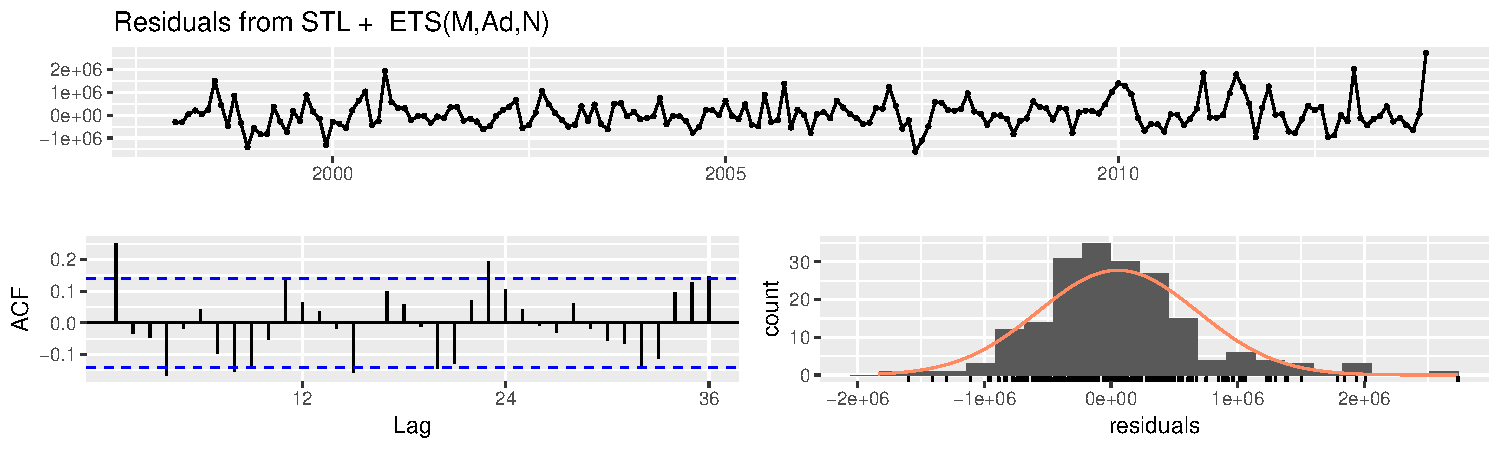
\includegraphics{Part-B-AS_files/figure-latex/unnamed-chunk-6-1.pdf}

Let's do deeper EDA on ts\_data and handle outlier using tsoutliers().

\begin{Shaded}
\begin{Highlighting}[]
\CommentTok{#disable scientific notation (ONLY RUN ONCE)}
\KeywordTok{options}\NormalTok{(}\DataTypeTok{scipen =} \DecValTok{99999}\NormalTok{)}

\KeywordTok{autoplot}\NormalTok{(ts_data) }\OperatorTok{+}
\KeywordTok{labs}\NormalTok{(}\DataTypeTok{title =} \StringTok{"Monthly Residential Power Usage"}\NormalTok{, }\DataTypeTok{subtitle =} \StringTok{"01/98 - 12/13"}\NormalTok{)}\OperatorTok{+}
\KeywordTok{theme_classic}\NormalTok{();}
\end{Highlighting}
\end{Shaded}

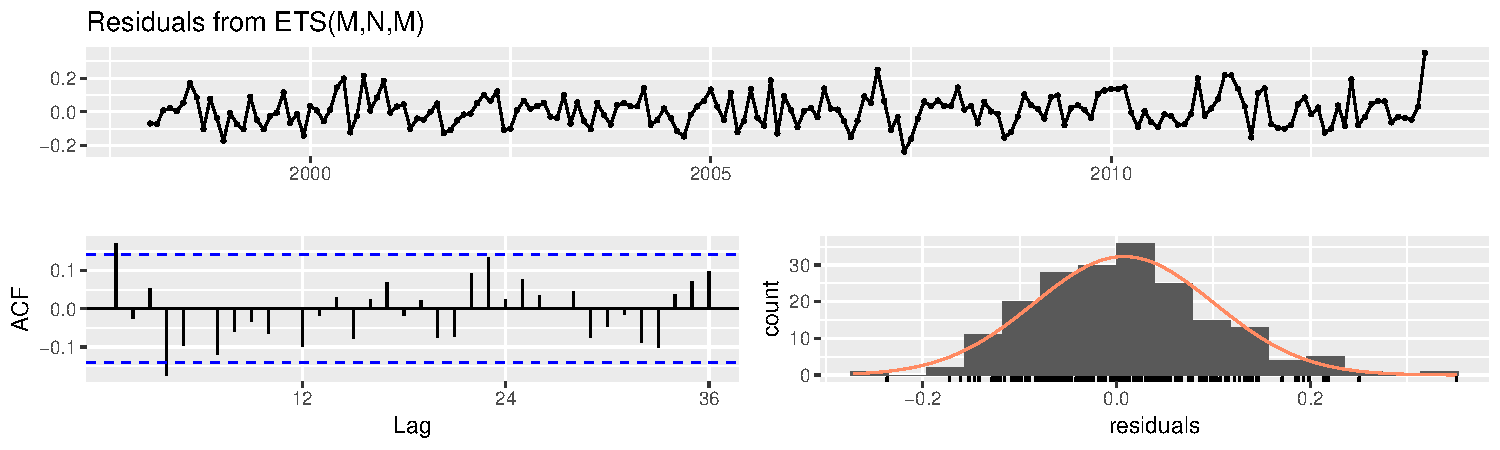
\includegraphics{Part-B-AS_files/figure-latex/unnamed-chunk-7-1.pdf}

\begin{Shaded}
\begin{Highlighting}[]
\KeywordTok{ggseasonplot}\NormalTok{(ts_data);}
\end{Highlighting}
\end{Shaded}

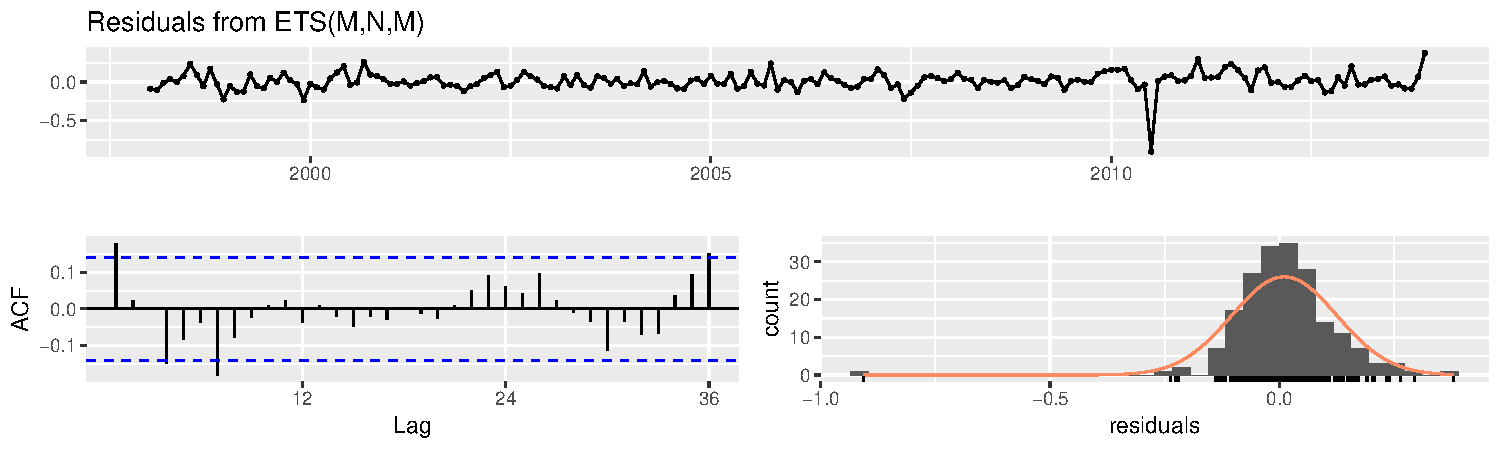
\includegraphics{Part-B-AS_files/figure-latex/unnamed-chunk-7-2.pdf}

\begin{Shaded}
\begin{Highlighting}[]
\KeywordTok{boxplot}\NormalTok{(ts_data}\OperatorTok{~}\KeywordTok{cycle}\NormalTok{(ts_data),}\DataTypeTok{xlab=}\StringTok{"Month"}\NormalTok{, }\DataTypeTok{ylab =} \StringTok{"Monthly Residential Power Usage"}\NormalTok{);}
\end{Highlighting}
\end{Shaded}

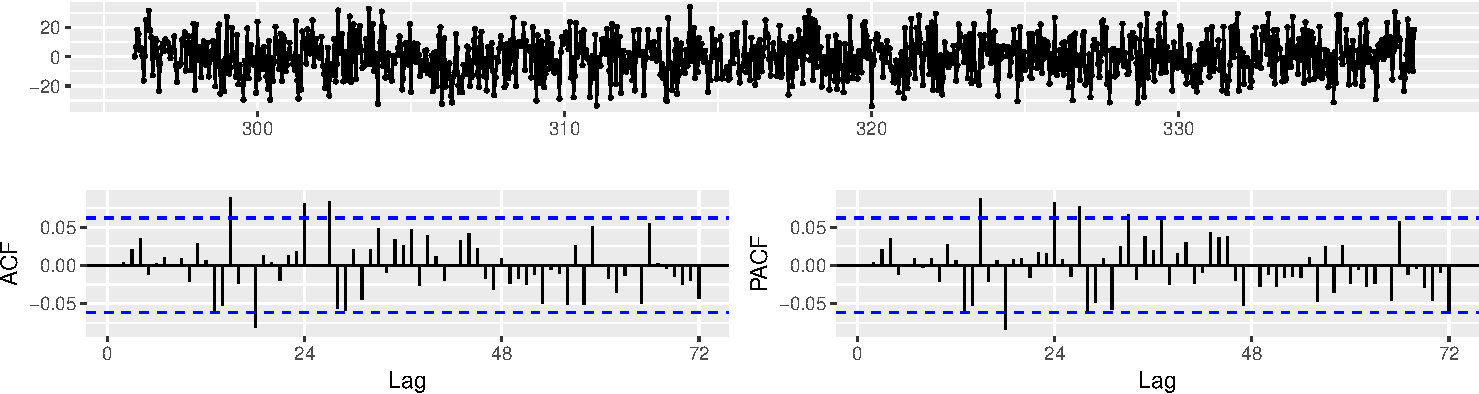
\includegraphics{Part-B-AS_files/figure-latex/unnamed-chunk-7-3.pdf}

\begin{Shaded}
\begin{Highlighting}[]
\KeywordTok{ggsubseriesplot}\NormalTok{(ts_data);}
\end{Highlighting}
\end{Shaded}

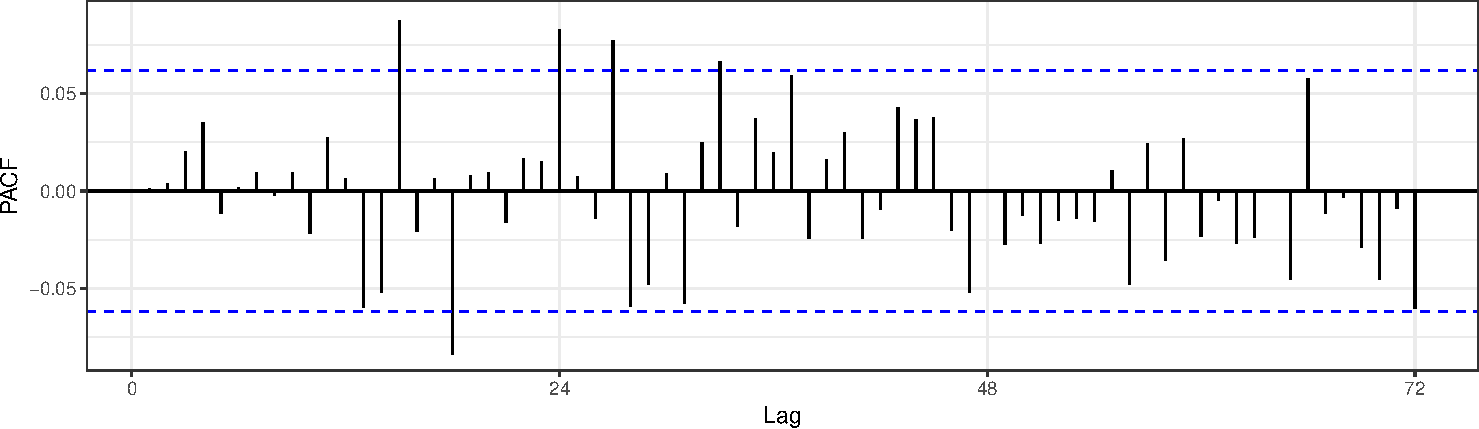
\includegraphics{Part-B-AS_files/figure-latex/unnamed-chunk-7-4.pdf}

\begin{Shaded}
\begin{Highlighting}[]
\KeywordTok{stl}\NormalTok{(ts_data, }\DataTypeTok{s.window =} \StringTok{'periodic'}\NormalTok{) }\OperatorTok\StringTok{ }\KeywordTok{autoplot}\NormalTok{();}
\end{Highlighting}
\end{Shaded}

\includegraphics{Part-B-AS_files/figure-latex/unnamed-chunk-7-5.pdf}

\begin{Shaded}
\begin{Highlighting}[]
\KeywordTok{ggAcf}\NormalTok{(ts_data);}
\end{Highlighting}
\end{Shaded}

\includegraphics{Part-B-AS_files/figure-latex/unnamed-chunk-7-6.pdf}

\begin{Shaded}
\begin{Highlighting}[]
\CommentTok{#Box.test(ts_data, type = c("Ljung-Box"))}


\CommentTok{# handling outlier}
\CommentTok{#fit <- nnetar(tsclean(ts_data))}
\NormalTok{outlier_func <-}\StringTok{ }\KeywordTok{tsoutliers}\NormalTok{(ts_data, }\DataTypeTok{iterate =} \DecValTok{2}\NormalTok{, }\DataTypeTok{lambda =} \StringTok{"auto"}\NormalTok{)}
\NormalTok{ts_data[outlier_func}\OperatorTok{$}\NormalTok{index] <-}\StringTok{ }\NormalTok{outlier_func}\OperatorTok{$}\NormalTok{replacements}
\end{Highlighting}
\end{Shaded}

Our initial plots reveal annual seasonality within this time series. The
box plot/seasonality plot actually reveals where power consumption
fluctuations occur within each of the cycke positions. We can speculate
that this could be due to there being no major Holidays that require
power draining decor plus we assume minimal AC usage during the cold
months.

We see power consumption increase between the months of June and August.
This must be tied to AC usage during the warmer months of a year and
finally power usage dips from September to Novemeber with a small spike
in December. We speculate that thisis due to transitioning out of
summer. The spike in December could be connected to the usage or Holiday
lights being kept on.

Within the overall TS plot, we see a dip in July 2010. This could be due
to a power outtage during a hot summer month. This can certainly be
considered to be an outlier within this TS. Using TSOutliers, we can
actually identify the index where our outliers may be. TSoutliers also
replaces the outlier using Box-Cox. If set lambda=auto, then TSoutliers
will automatically perform Box-Cox transformation.

The ACF plot shows that autocorrelations are well outside the
significant space indicating the series is not white noise,
non-stationary.

\section*{Data Model}\label{b-model}
\addcontentsline{toc}{section}{Data Model}

\subsection{Model \#1: ARIMA}\label{model-1-arima}

\begin{Shaded}
\begin{Highlighting}[]
\NormalTok{arima_model <-}\StringTok{ }\KeywordTok{auto.arima}\NormalTok{(ts_data)}

\NormalTok{arima_model <-}\StringTok{ }\KeywordTok{forecast}\NormalTok{(arima_model, }\DataTypeTok{h=}\DecValTok{12}\NormalTok{)}

\KeywordTok{autoplot}\NormalTok{(arima_model) }\OperatorTok{+}\StringTok{ }\KeywordTok{autolayer}\NormalTok{(}\KeywordTok{fitted}\NormalTok{(arima_model))}
\end{Highlighting}
\end{Shaded}

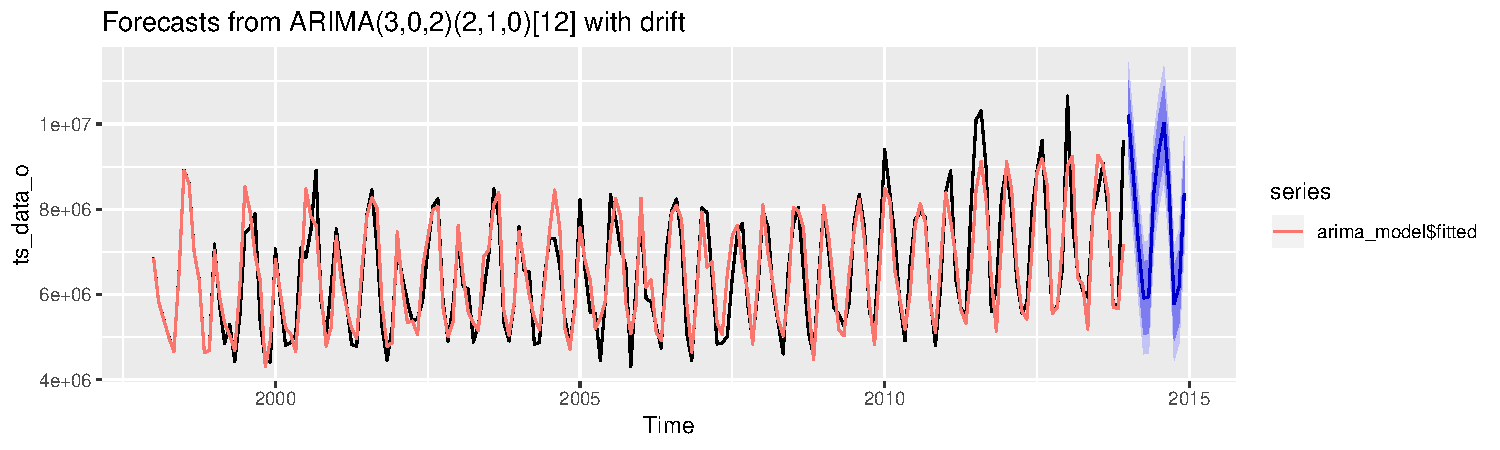
\includegraphics{Part-B-AS_files/figure-latex/unnamed-chunk-8-1.pdf}

\begin{Shaded}
\begin{Highlighting}[]
\KeywordTok{checkresiduals}\NormalTok{(arima_model)}
\end{Highlighting}
\end{Shaded}

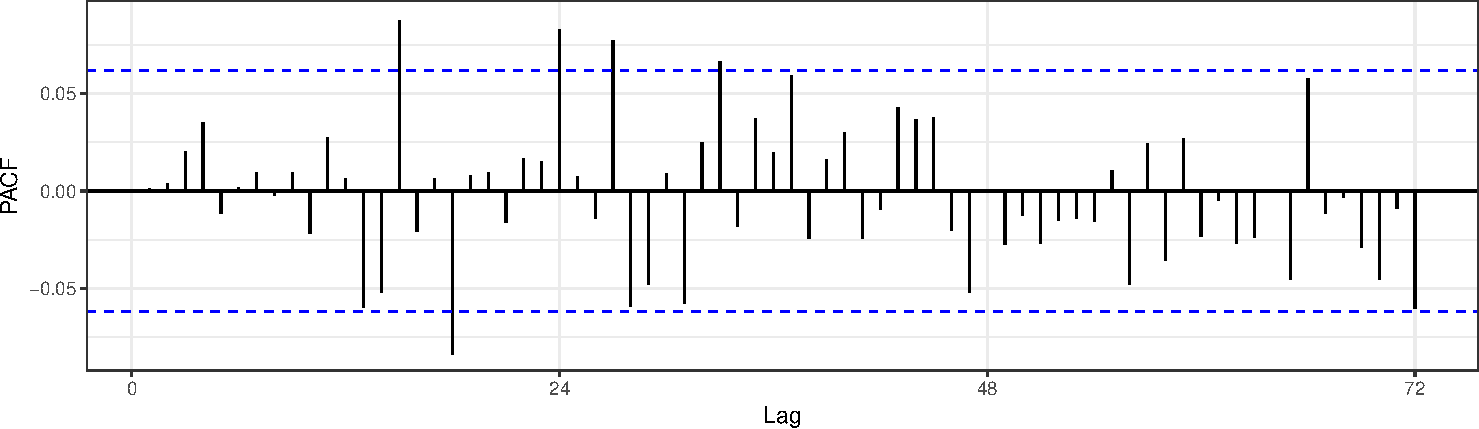
\includegraphics{Part-B-AS_files/figure-latex/unnamed-chunk-8-2.pdf}

\begin{verbatim}
FALSE 
FALSE   Ljung-Box test
FALSE 
FALSE data:  Residuals from ARIMA(3,0,2)(2,1,0)[12] with drift
FALSE Q* = 12.555, df = 16, p-value = 0.705
FALSE 
FALSE Model df: 8.   Total lags used: 24
\end{verbatim}

\subsection{Model \#2: STL (no-demped) -
MNN}\label{model-2-stl-no-demped---mnn}

\begin{Shaded}
\begin{Highlighting}[]
\CommentTok{#stlf - etsmodel estimation --- M,N,N is chosen.}
\NormalTok{stl_ndemp <-}\StringTok{ }\KeywordTok{stlf}\NormalTok{(ts_data, }\DataTypeTok{s.window =} \StringTok{"periodic"}\NormalTok{, }\DataTypeTok{robust=}\OtherTok{TRUE}\NormalTok{, }\DataTypeTok{h =} \DecValTok{12}\NormalTok{)}

\CommentTok{# forecast plot}
\KeywordTok{autoplot}\NormalTok{(stl_ndemp) }\OperatorTok{+}\StringTok{ }\KeywordTok{autolayer}\NormalTok{(}\KeywordTok{fitted}\NormalTok{(stl_ndemp))}
\end{Highlighting}
\end{Shaded}

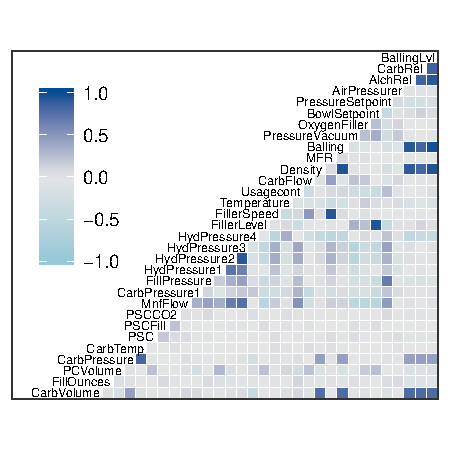
\includegraphics{Part-B-AS_files/figure-latex/unnamed-chunk-9-1.pdf}

\begin{Shaded}
\begin{Highlighting}[]
\KeywordTok{checkresiduals}\NormalTok{(stl_ndemp)}
\end{Highlighting}
\end{Shaded}

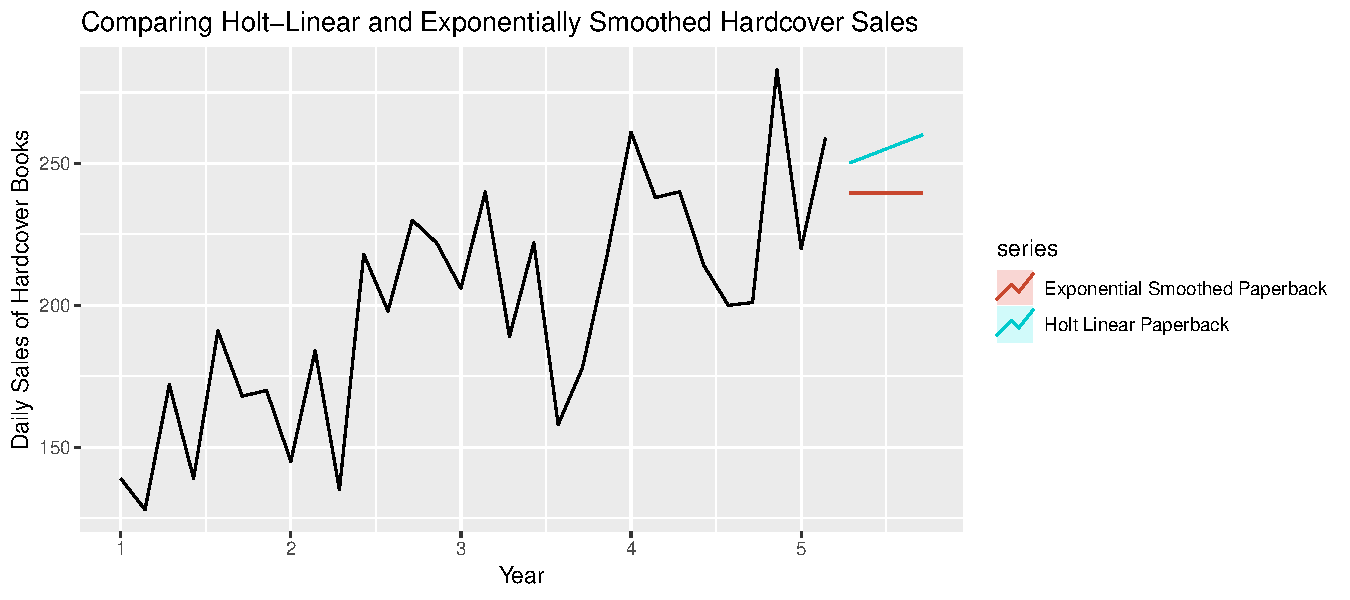
\includegraphics{Part-B-AS_files/figure-latex/unnamed-chunk-9-2.pdf}

\begin{verbatim}
FALSE 
FALSE   Ljung-Box test
FALSE 
FALSE data:  Residuals from STL +  ETS(M,N,N)
FALSE Q* = 65.934, df = 22, p-value = 0.00000284
FALSE 
FALSE Model df: 2.   Total lags used: 24
\end{verbatim}

\subsection{Model \#2-2: STL (demped) -
MAdN}\label{model-2-2-stl-demped---madn}

\begin{Shaded}
\begin{Highlighting}[]
\CommentTok{#stlf - etsmodel estimation --- M, Ad, N is chosen.}
\NormalTok{stl_demp <-}\StringTok{ }\KeywordTok{stlf}\NormalTok{(ts_data, }\DataTypeTok{damped=}\OtherTok{TRUE}\NormalTok{, }\DataTypeTok{s.window =} \StringTok{"periodic"}\NormalTok{, }\DataTypeTok{robust=}\OtherTok{TRUE}\NormalTok{, }\DataTypeTok{h =} \DecValTok{12}\NormalTok{)}

\CommentTok{# forecast plot}
\KeywordTok{autoplot}\NormalTok{(stl_demp) }\OperatorTok{+}\StringTok{ }\KeywordTok{autolayer}\NormalTok{(}\KeywordTok{fitted}\NormalTok{(stl_demp))}
\end{Highlighting}
\end{Shaded}

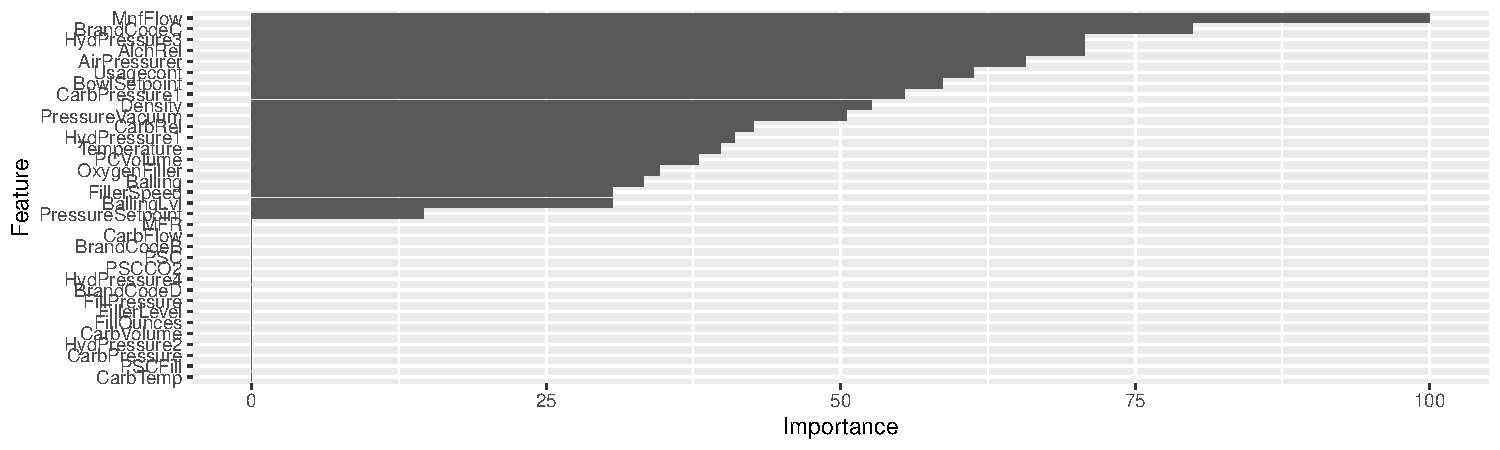
\includegraphics{Part-B-AS_files/figure-latex/unnamed-chunk-10-1.pdf}

\begin{Shaded}
\begin{Highlighting}[]
\KeywordTok{checkresiduals}\NormalTok{(stl_demp)}
\end{Highlighting}
\end{Shaded}

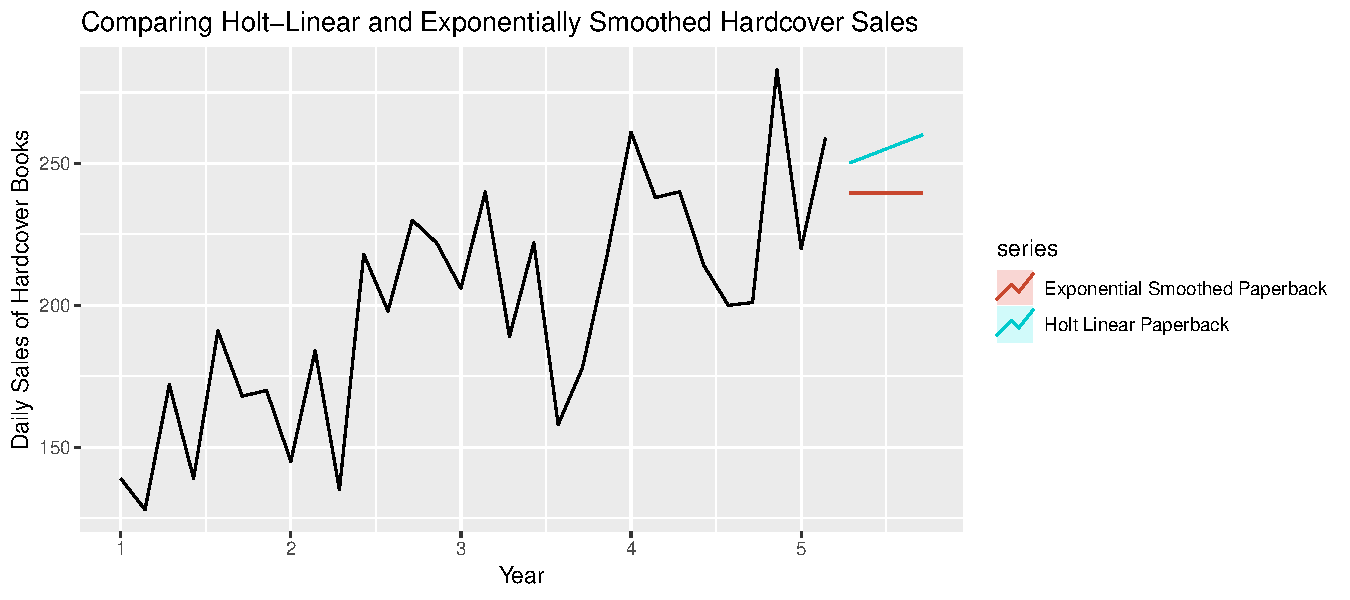
\includegraphics{Part-B-AS_files/figure-latex/unnamed-chunk-10-2.pdf}

\begin{verbatim}
FALSE 
FALSE   Ljung-Box test
FALSE 
FALSE data:  Residuals from STL +  ETS(M,Ad,N)
FALSE Q* = 63.375, df = 19, p-value = 0.000001119
FALSE 
FALSE Model df: 5.   Total lags used: 24
\end{verbatim}

\subsection{Model \#3: ets - MNM}\label{model-3-ets---mnm}

\begin{Shaded}
\begin{Highlighting}[]
\CommentTok{# ETS models - MNM}
\NormalTok{ets_model <-}\StringTok{ }\KeywordTok{ets}\NormalTok{(ts_data)}

\CommentTok{# forecast plot}
\KeywordTok{autoplot}\NormalTok{(}\KeywordTok{forecast}\NormalTok{(ets_model, }\DataTypeTok{h=}\DecValTok{12}\NormalTok{)) }\OperatorTok{+}\StringTok{ }\KeywordTok{autolayer}\NormalTok{(}\KeywordTok{fitted}\NormalTok{(ets_model))}
\end{Highlighting}
\end{Shaded}

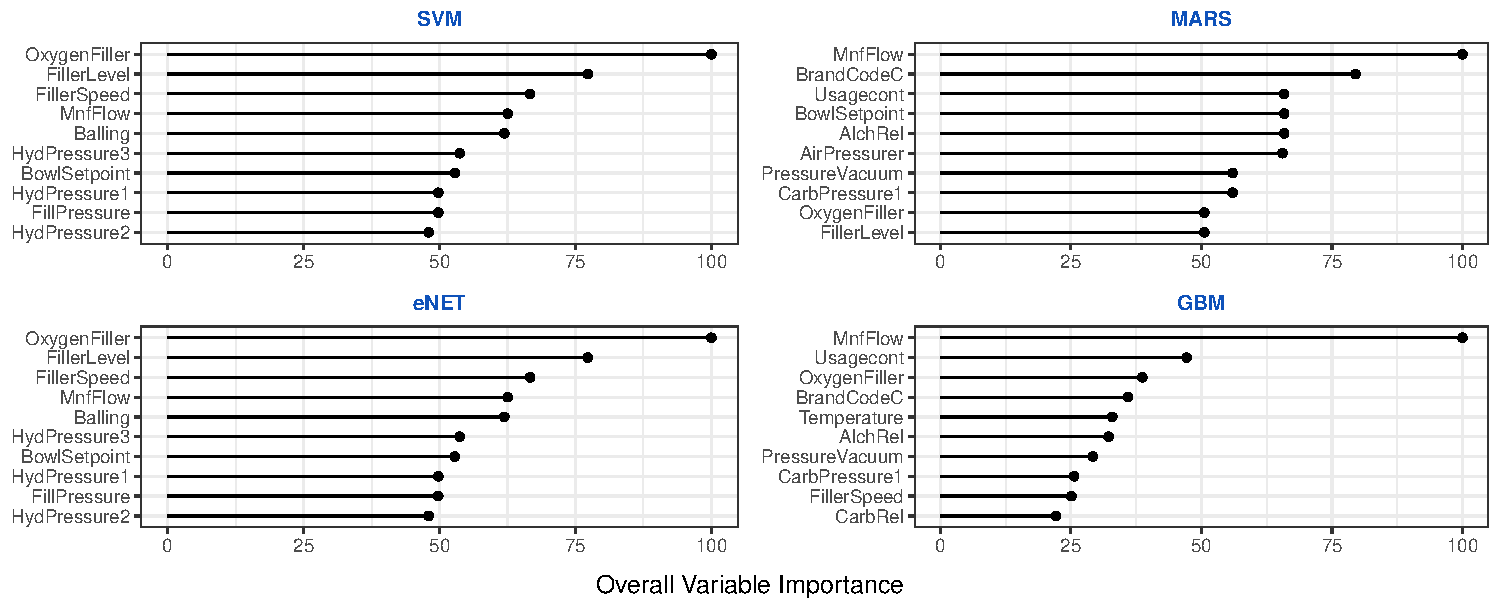
\includegraphics{Part-B-AS_files/figure-latex/unnamed-chunk-11-1.pdf}

\begin{Shaded}
\begin{Highlighting}[]
\KeywordTok{checkresiduals}\NormalTok{(ets_model)}
\end{Highlighting}
\end{Shaded}

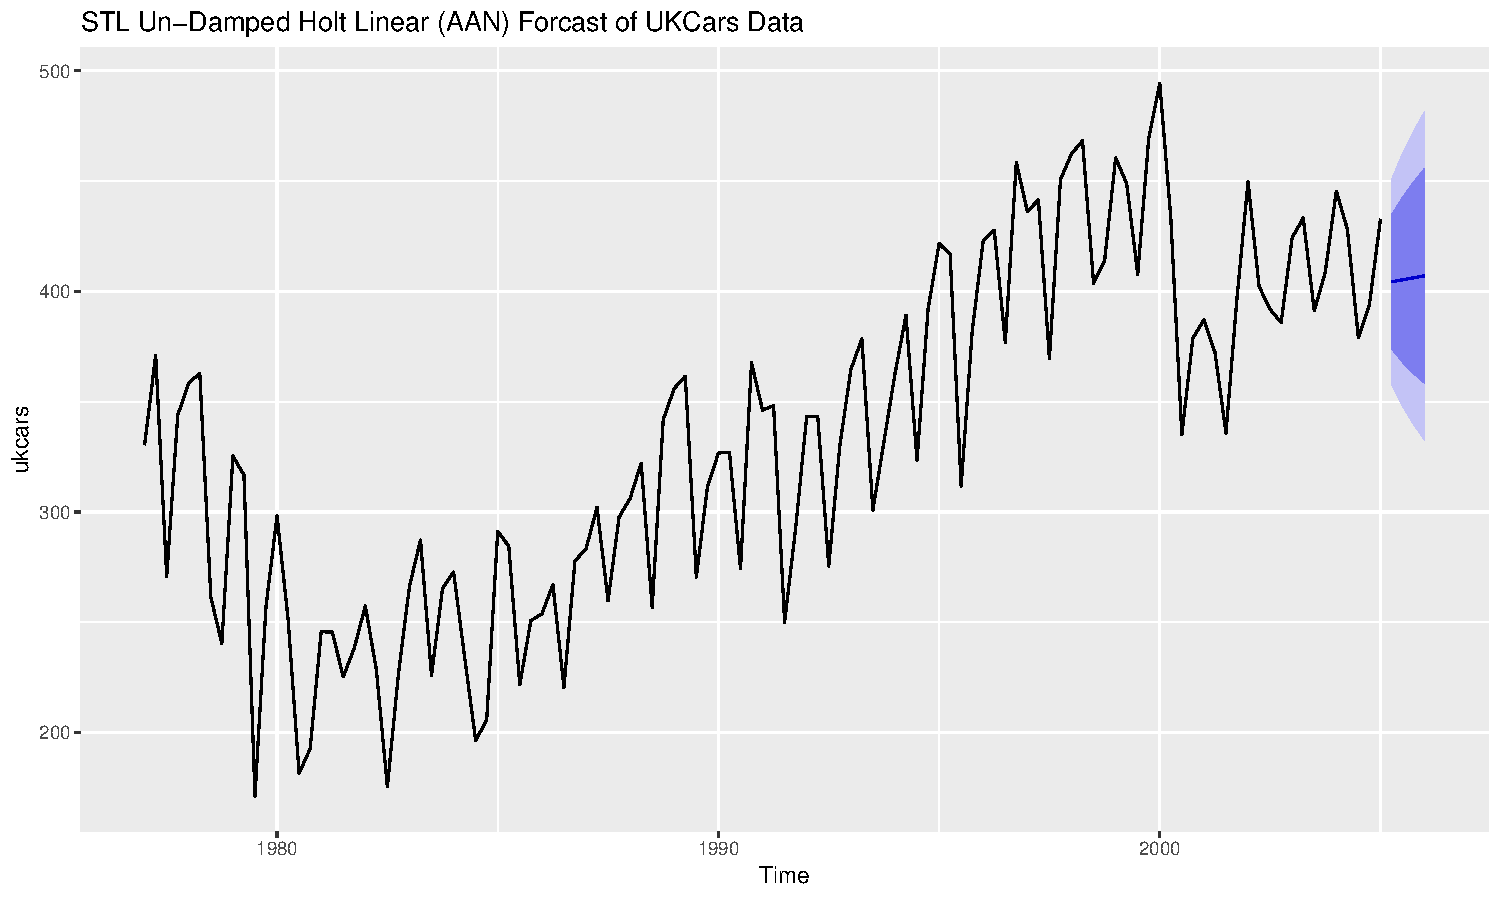
\includegraphics{Part-B-AS_files/figure-latex/unnamed-chunk-11-2.pdf}

\begin{verbatim}
FALSE 
FALSE   Ljung-Box test
FALSE 
FALSE data:  Residuals from ETS(M,N,M)
FALSE Q* = 32.042, df = 10, p-value = 0.000394
FALSE 
FALSE Model df: 14.   Total lags used: 24
\end{verbatim}

\subsection{Model \#4: Regression}\label{model-4-regression}

\begin{Shaded}
\begin{Highlighting}[]
\NormalTok{fit.reg <-}\StringTok{ }\KeywordTok{tslm}\NormalTok{(ts_data }\OperatorTok{~}\StringTok{ }\NormalTok{trend }\OperatorTok{+}\StringTok{ }\NormalTok{season)}
\NormalTok{reg_model <-}\StringTok{ }\KeywordTok{forecast}\NormalTok{(fit.reg, }\DataTypeTok{h =} \DecValTok{12}\NormalTok{)}

\CommentTok{# forecast plot}
\KeywordTok{autoplot}\NormalTok{(reg_model) }\OperatorTok{+}\StringTok{ }\KeywordTok{autolayer}\NormalTok{(}\KeywordTok{fitted}\NormalTok{(reg_model))}
\end{Highlighting}
\end{Shaded}

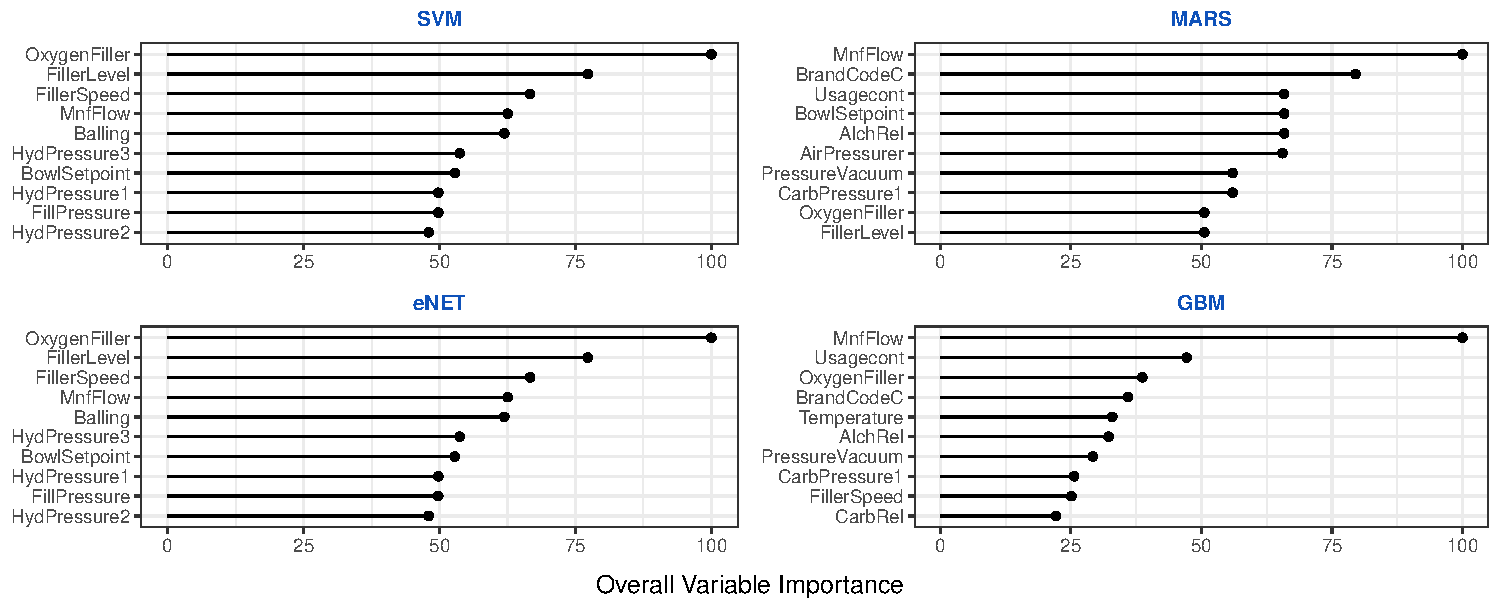
\includegraphics{Part-B-AS_files/figure-latex/unnamed-chunk-12-1.pdf}

\begin{Shaded}
\begin{Highlighting}[]
\KeywordTok{checkresiduals}\NormalTok{(reg_model)}
\end{Highlighting}
\end{Shaded}

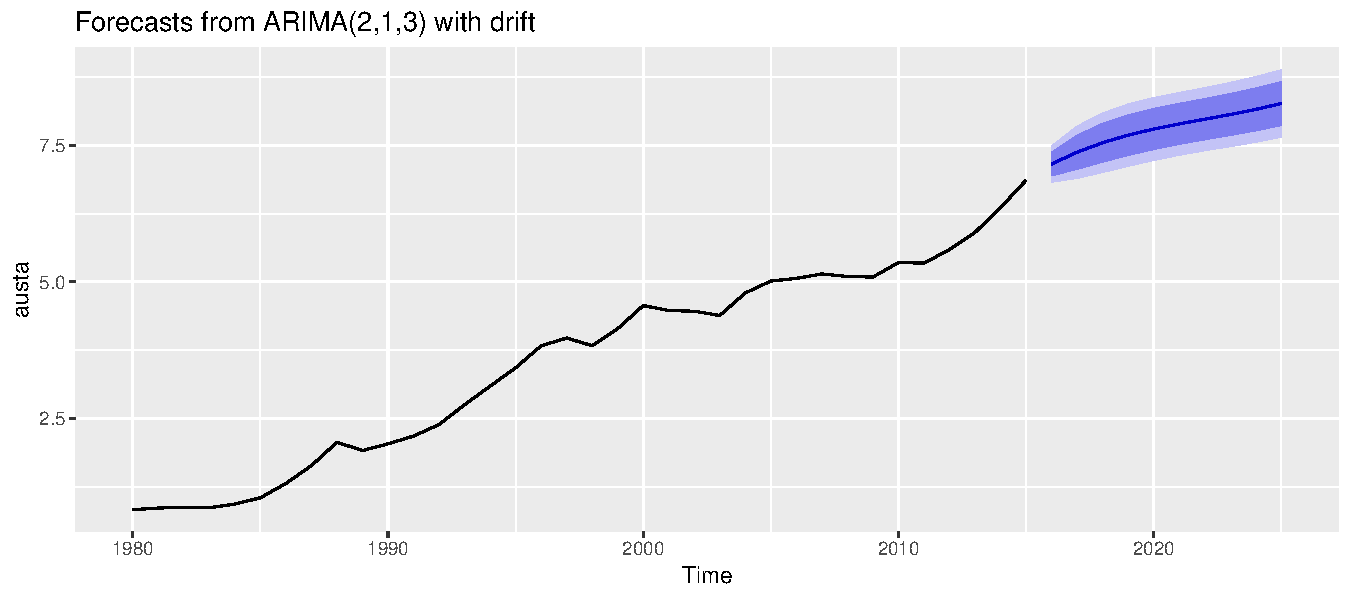
\includegraphics{Part-B-AS_files/figure-latex/unnamed-chunk-12-2.pdf}

\begin{verbatim}
FALSE 
FALSE   Ljung-Box test
FALSE 
FALSE data:  Residuals from Linear regression model
FALSE Q* = 80.001, df = 11, p-value = 0.000000000001475
FALSE 
FALSE Model df: 13.   Total lags used: 24
\end{verbatim}

\subsection{Model \#5: TBATS}\label{model-5-tbats}

\begin{Shaded}
\begin{Highlighting}[]
\NormalTok{fit.tbats <-}\StringTok{ }\KeywordTok{tbats}\NormalTok{(ts_data)}
\NormalTok{tbats_model <-}\StringTok{ }\KeywordTok{forecast}\NormalTok{(fit.tbats, }\DataTypeTok{h =} \DecValTok{12}\NormalTok{)}

\CommentTok{# forecast plot}
\KeywordTok{autoplot}\NormalTok{(tbats_model) }\OperatorTok{+}\StringTok{ }\KeywordTok{autolayer}\NormalTok{(}\KeywordTok{fitted}\NormalTok{(tbats_model))}
\end{Highlighting}
\end{Shaded}

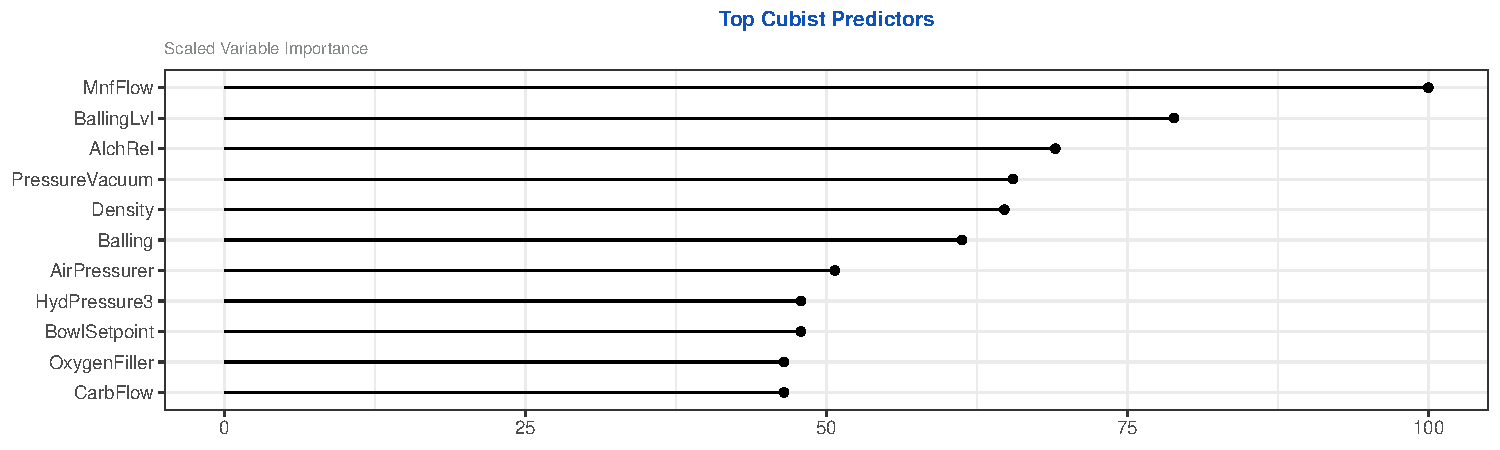
\includegraphics{Part-B-AS_files/figure-latex/unnamed-chunk-13-1.pdf}

\begin{Shaded}
\begin{Highlighting}[]
\KeywordTok{checkresiduals}\NormalTok{(tbats_model)}
\end{Highlighting}
\end{Shaded}

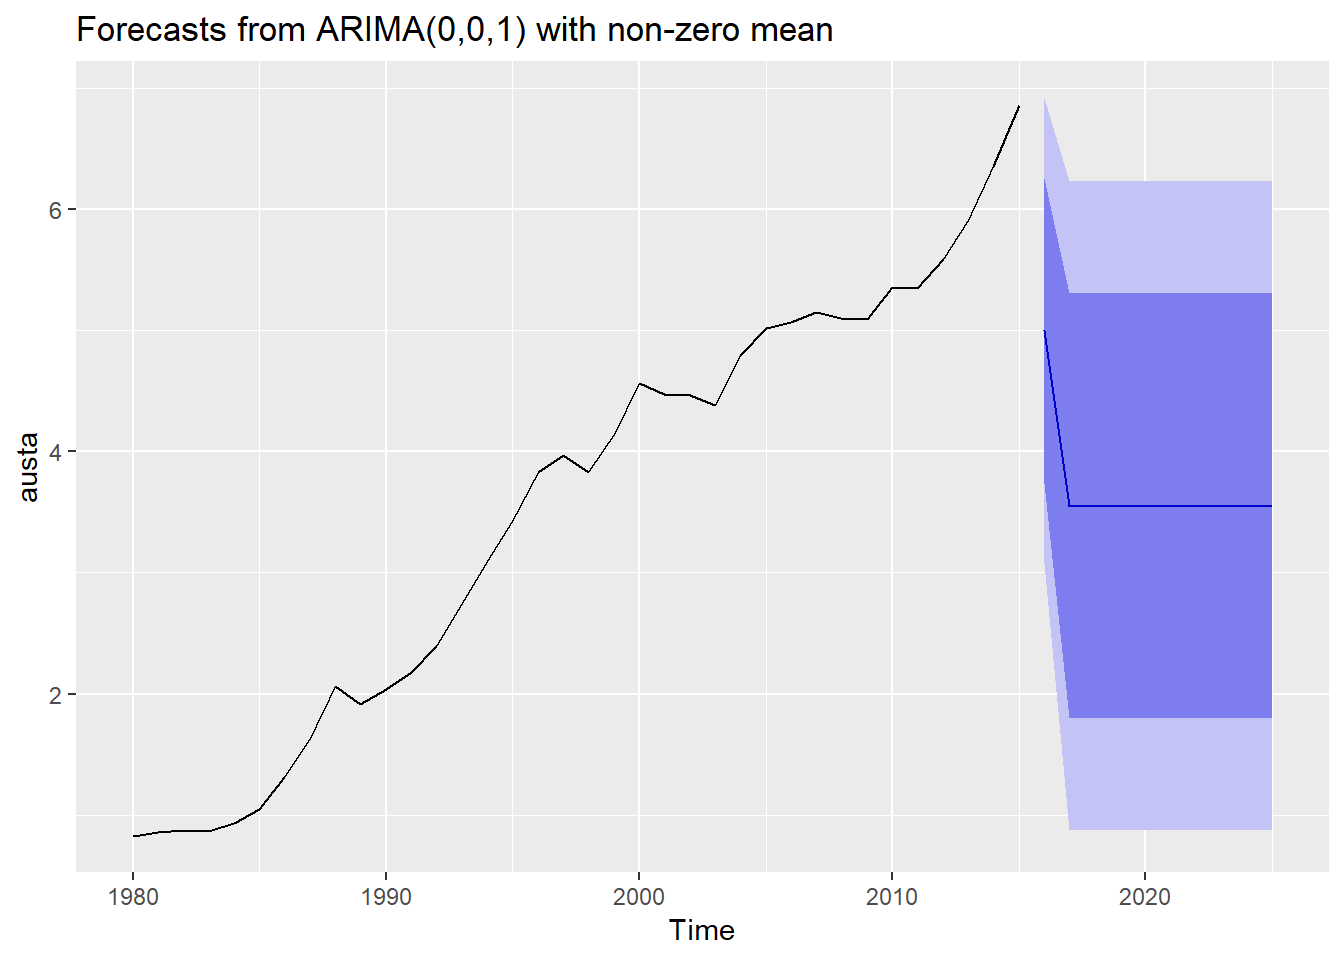
\includegraphics{Part-B-AS_files/figure-latex/unnamed-chunk-13-2.pdf}

\begin{verbatim}
FALSE 
FALSE   Ljung-Box test
FALSE 
FALSE data:  Residuals from TBATS(0.002, {0,1}, -, {<12,5>})
FALSE Q* = 26.054, df = 7, p-value = 0.0004925
FALSE 
FALSE Model df: 17.   Total lags used: 24
\end{verbatim}

\subsection{Accuracy of Models}\label{accuracy-of-models}

\begin{Shaded}
\begin{Highlighting}[]
\KeywordTok{accuracy}\NormalTok{(arima_model);}
\end{Highlighting}
\end{Shaded}

\begin{verbatim}
FALSE                     ME     RMSE      MAE        MPE     MAPE      MASE
FALSE Training set -8455.077 589381.7 427752.5 -0.7944782 6.475365 0.6904053
FALSE                      ACF1
FALSE Training set 0.0006090194
\end{verbatim}

\begin{Shaded}
\begin{Highlighting}[]
\KeywordTok{accuracy}\NormalTok{(stl_ndemp);}
\end{Highlighting}
\end{Shaded}

\begin{verbatim}
FALSE                    ME     RMSE      MAE         MPE     MAPE      MASE
FALSE Training set 56926.03 633571.7 460713.4 -0.03288687 6.945185 0.7436052
FALSE                   ACF1
FALSE Training set 0.2570241
\end{verbatim}

\begin{Shaded}
\begin{Highlighting}[]
\KeywordTok{accuracy}\NormalTok{(stl_demp);}
\end{Highlighting}
\end{Shaded}

\begin{verbatim}
FALSE                    ME     RMSE      MAE         MPE     MAPE      MASE
FALSE Training set 54337.68 631081.9 458777.5 -0.07364717 6.937249 0.7404807
FALSE                   ACF1
FALSE Training set 0.2528558
\end{verbatim}

\begin{Shaded}
\begin{Highlighting}[]
\KeywordTok{accuracy}\NormalTok{(ets_model);}
\end{Highlighting}
\end{Shaded}

\begin{verbatim}
FALSE                    ME     RMSE      MAE         MPE     MAPE      MASE
FALSE Training set 45241.77 628252.5 481520.9 -0.04000239 7.277118 0.7771892
FALSE                   ACF1
FALSE Training set 0.1927438
\end{verbatim}

\begin{Shaded}
\begin{Highlighting}[]
\KeywordTok{accuracy}\NormalTok{(reg_model);}
\end{Highlighting}
\end{Shaded}

\begin{verbatim}
FALSE                                ME     RMSE      MAE        MPE     MAPE
FALSE Training set -0.00000000001455192 637832.8 480849.1 -0.8253442 7.286874
FALSE                   MASE      ACF1
FALSE Training set 0.7761049 0.3597939
\end{verbatim}

\begin{Shaded}
\begin{Highlighting}[]
\KeywordTok{accuracy}\NormalTok{(tbats_model)}
\end{Highlighting}
\end{Shaded}

\begin{verbatim}
FALSE                    ME     RMSE      MAE       MPE    MAPE      MASE
FALSE Training set 97092.89 577485.8 433659.7 0.7290721 6.54268 0.6999398
FALSE                    ACF1
FALSE Training set 0.01196249
\end{verbatim}

Out of the models we built, we can make some preliminary observations.
The residuals for each of our models does not have a major deviance from
normality, however Model \#1: ARIMA residuals do not have an extended
number of bins distorting the normality proximity but we can say it is
still fairly normally distributed.

The residual ACF plots show residual autocorrelations for each of our
models. Model \#1: ARIMA has less autocorrelation than the other three
models. Model 1 is well within the 95\% limits indicated by the dotted
blue lines.

If we examine the Ljung-Box test results for our models, the only model
with a p-value \textgreater{} 0.05 is Model \#1: ARIMA. This implies
that the residuals from other models are not independent, hence not
white noise.

In contrast, when we first attempted the analysis by building models
without handling outlier (2010 Jul), the only model with a p-value
\textless{} 0.05 was Model \#3: ets - MNN and hence we accepted all the
other models except for \#3.

Handling 1 outlier dramatically changed the outcome of Ljung-Box test.

\section*{Forecast}\label{b-forecast}
\addcontentsline{toc}{section}{Forecast}

We will implement a cross validation method of testing for h=12. The
process randomly chooses 12 points to measure and take the average of
RMSEs. By definition, a lower RMSE on test set is attributed with a
better forecast on unseen data. We only accepted Model \#1 from
Ljung-Box test and hence it is our final choice.

\subsection{Model \#1: ARIMA}\label{model-1-arima-1}

\begin{Shaded}
\begin{Highlighting}[]
\NormalTok{arima_cv <-}\StringTok{ }\ControlFlowTok{function}\NormalTok{(x, h)\{}\KeywordTok{forecast}\NormalTok{(}\KeywordTok{Arima}\NormalTok{(x, }\DataTypeTok{order =} \KeywordTok{c}\NormalTok{(}\DecValTok{3}\NormalTok{, }\DecValTok{0}\NormalTok{, }\DecValTok{2}\NormalTok{), }\DataTypeTok{seasonal =} \KeywordTok{c}\NormalTok{(}\DecValTok{2}\NormalTok{, }\DecValTok{1}\NormalTok{, }\DecValTok{0}\NormalTok{), }\DataTypeTok{include.drift =} \OtherTok{TRUE}\NormalTok{), }\DataTypeTok{h=}\NormalTok{h)\}}

\NormalTok{e <-}\StringTok{ }\KeywordTok{tsCV}\NormalTok{(ts_data, arima_cv, }\DataTypeTok{h=}\DecValTok{12}\NormalTok{)}

\KeywordTok{sqrt}\NormalTok{(}\KeywordTok{mean}\NormalTok{(e}\OperatorTok{^}\DecValTok{2}\NormalTok{, }\DataTypeTok{na.rm=}\OtherTok{TRUE}\NormalTok{))}
\end{Highlighting}
\end{Shaded}

\begin{verbatim}
FALSE [1] 725175
\end{verbatim}

Using Time series cross-validation, we compute RMSE on testset (h=12).
We would have to pick the model with the lowest RMSE on test set as our
final model if we had more than 1 model to compare. In our case, since
we only have 1 model left after Ljung test, we have no choice but to
pick seasonal ARIMA model as our final choice. Cross-validation test
shows that RMSE on test is around 720k when RMSE on training is around
589k. We can conclude the model is not necessarily overfitted. Given
that MAPE on training is less than 7, it is not a suprising result.

\section*{Discussion}\label{b-discussion}
\addcontentsline{toc}{section}{Discussion}

In our first phased implicit analysis, which is not recorded on this
Rmd, where outlier (2010 - Jul) was not handled, STL - ANN was the best
model in terms of RMSE on test set. As outlier was handled, on the other
hand, STL models became invalid predictors as residuals were
autocorrelated. We learned that handling outlier, even if it is just one
data point, makes the result of modelling outcome completely.


\end{document}
